\documentclass[a4paper, 11pt]{article}
\usepackage{comment} % enables the use of multi-line comments (\ifx \fi) 
\usepackage{lipsum} %This package just generates Lorem Ipsum filler text. 
\usepackage{fullpage} % changes the margin
\usepackage{outline}
\usepackage{pmgraph}
\usepackage[utf8x]{inputenc}
\usepackage[T1]{fontenc}
\usepackage{esvect}
\usepackage{amsmath}
\usepackage{bm}
\usepackage{mathtools}
\usepackage{tcolorbox}
\usepackage{longtable}
\usepackage{physics}
%\usepackage[document]{ragged2e}
\usepackage{color}
\usepackage{multicol}
\usepackage{bm}
\usepackage{graphicx}
\usepackage{setspace}
\usepackage{amssymb}
\usepackage{amsmath}
\usepackage[nottoc]{tocbibind}
\usepackage[normalem]{ulem}
\usepackage{caption}
\usepackage{subcaption}

\begin{document}
%Header-Make sure you update this information!!!!
\noindent
\large\textbf{Assignment Report} \hfill \textbf{Ramy Tanios} \\
\normalsize MECH764 \hfill 201404444 \\
Prof. Fadl Moukalled \hfill \\ \hfill Due Date: 12/4/2018

\section*{Introduction}
In this report, I will be presenting the results of the finite volume method applied to the two dimensional diffusion-convection equation $-\nabla.(\Gamma^{\phi}\nabla\phi)+\nabla.(\rho\mathbf{v}\phi)=S^{\phi}$, where $S^{\phi}$ is the source term, $\rho$ is the density of the fluid, $\Gamma^{\phi}$ is the diffusivity, $\mathbf{v}$ is the fluid's velocity field and $\phi$ is the variable to be solved for. In this assignment, we restrict to the pure convection equation by setting $\Gamma^{\phi}$ and $S^{\phi}$ to $0$. Two convection schemes will be implemented: the \textbf{upwind} scheme and the \textbf{smart} scheme, on a two dimensional square domain with known velocity field \textbf{v}.
%----------------
\section*{Implementation}
The method is implemented using fortran90. The main program \textit{main.f90} calls the following subroutines: \textit{allocateArrays.f90, transfiniteInterpolation.f90, geometricQuantities.f90, surfaceVectors.f90, getFields.f90, getDiffusiveCoeff.f90, getConvectiveCoeff.f90} and the solver \textit{iterativeSolver.f90} . \\
Most importantly, the subroutine \textit{getDiffusiveCoeff.f90} adds the contribution of the diffusion term to the coefficients $a_E, a_W, a_S, a_N, a_C$ and $b_C$ whereas \textit{getConvectiveCoeff.f90} adds to them the contribution of the convection term. Finally, \textit{iterativeSolver.f90} solves for the variable $\phi$ using the \textbf{TDMA} method, applied to lines of constant indexing $i$ and $j$ in order to get a tridiagonal matrix for the system of equations $\textbf{A}\phi=\textbf{b}$. \\ 
Also, using the command \textit{call system("python plot.py")}, the main program will call a python script that uses the \textit{matplotlib} library for plotting the results.\\
Now as for the variables, a logical variable is declared in the main program named \textit{smartSchemeS0lver}. If the user wants to solve the convection equation using the upwind scheme, this variable is set to false. On the other hand, if the user wants to use the smart scheme with the deferred correction approach, the \textit{smartSchemeS0lver} variable is set to true.\\
In the module \textit{fields.mod}, the user can change the velocity field function, the diffusivity field distribution and may add a source term to the equation to be solved. Finally, the boundary conditions of the problem are initialized in the module \textit{boundaryConditions.mod} . In that module, the user can change and set the desired boundary conditions. Note that all the variables in that module are declared as one dimensional arrays of size $4$, where the first element corresponds the boundary condition at the north boundary, the second for the east boundary, the third for the south boundary and finally the fourth element for the east boundary of the domain.
%----------------
\section*{Results}
In this section, results for the two convection schemes will be presented for the case where $\textbf{v}=\cos\frac{\pi}{4}\textbf{i}+\sin\frac{\pi}{4}\textbf{j}$. The boundary conditions provided are two inlet boundary conditions and two outlets. The west and south boundaries are inlets with $\phi_{in}$ is $0$ at the west boundary and $1$ at the south on. The other two boundaries are outlets. The value of the variable $\phi$ is plotted across the computational domain. We can notice from the plots that the upwind scheme does not provide much accuracy in comparison with the smart scheme, where more accuracy is attained however with a little bit of oscillations of the solution near the interface between the two flows of values $0$ and $1$.
\begin{figure}[h]
\centering
\begin{subfigure}{0.5\textwidth}
  \centering
  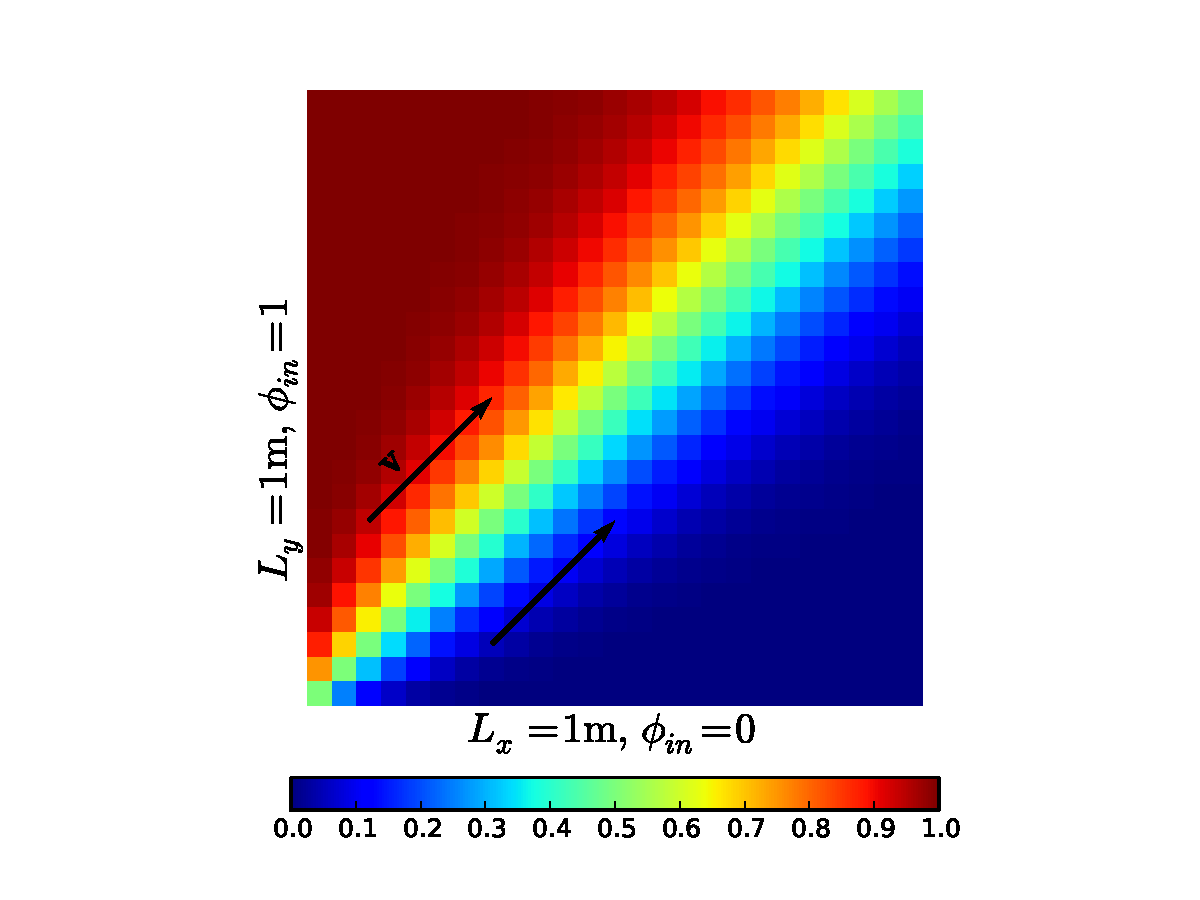
\includegraphics[width=1\linewidth]{up26.pdf}
  \caption{The upwind scheme.}
  \label{fig:sub1}
\end{subfigure}%
\begin{subfigure}{0.5\textwidth}
  \centering
  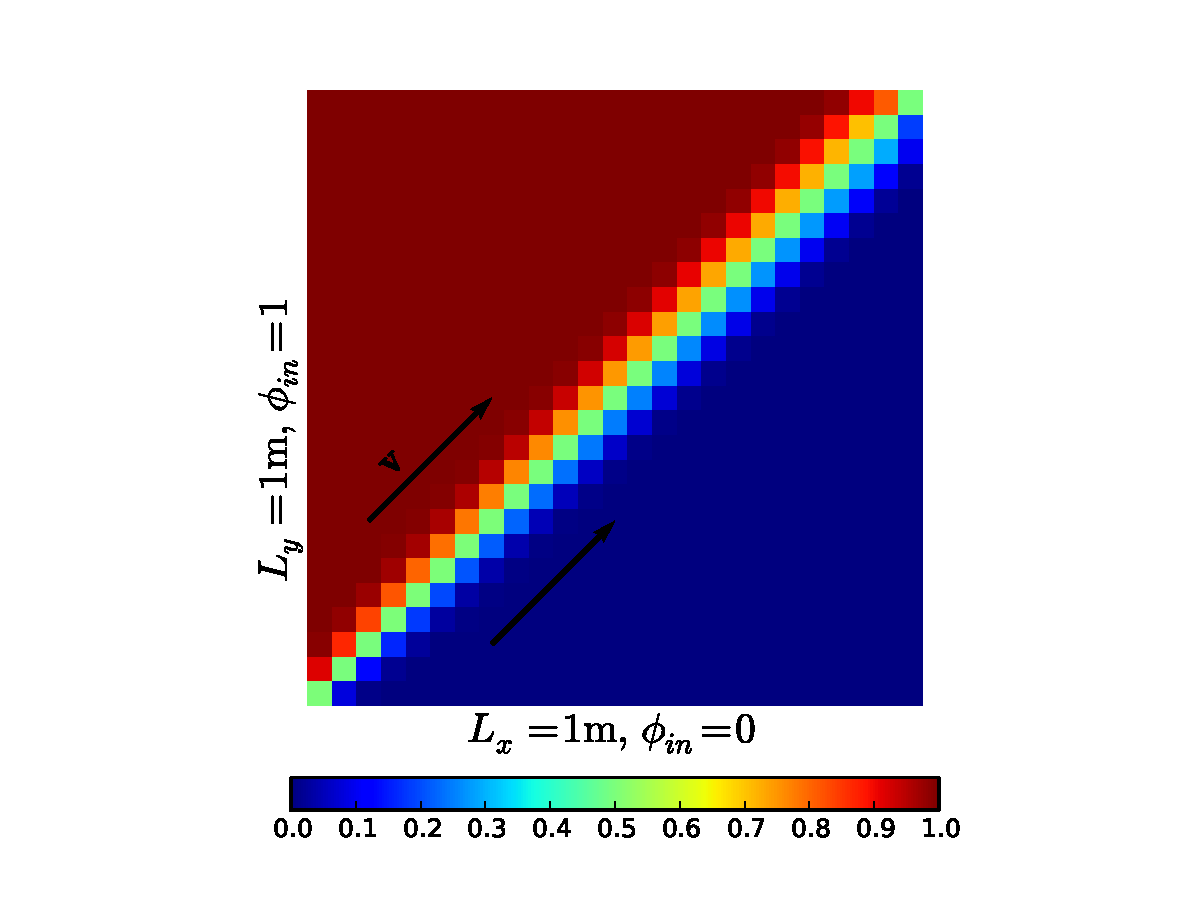
\includegraphics[width=1\linewidth]{smart26.pdf}
  \caption{The smart scheme.}
  \label{fig:sub2}
\end{subfigure}
\caption{The variable $\phi$ distribution over the computational domain using a grid size of 25x25 for the upwind and smart convection schemes and velocity field $\textbf{v}=\cos\frac{\pi}{4}\textbf{i}+\sin\frac{\pi}{4}\textbf{j}$.}
\label{fig:sub2}
\end{figure}

\begin{figure}[h]
\centering
\begin{subfigure}{0.5\textwidth}
  \centering
  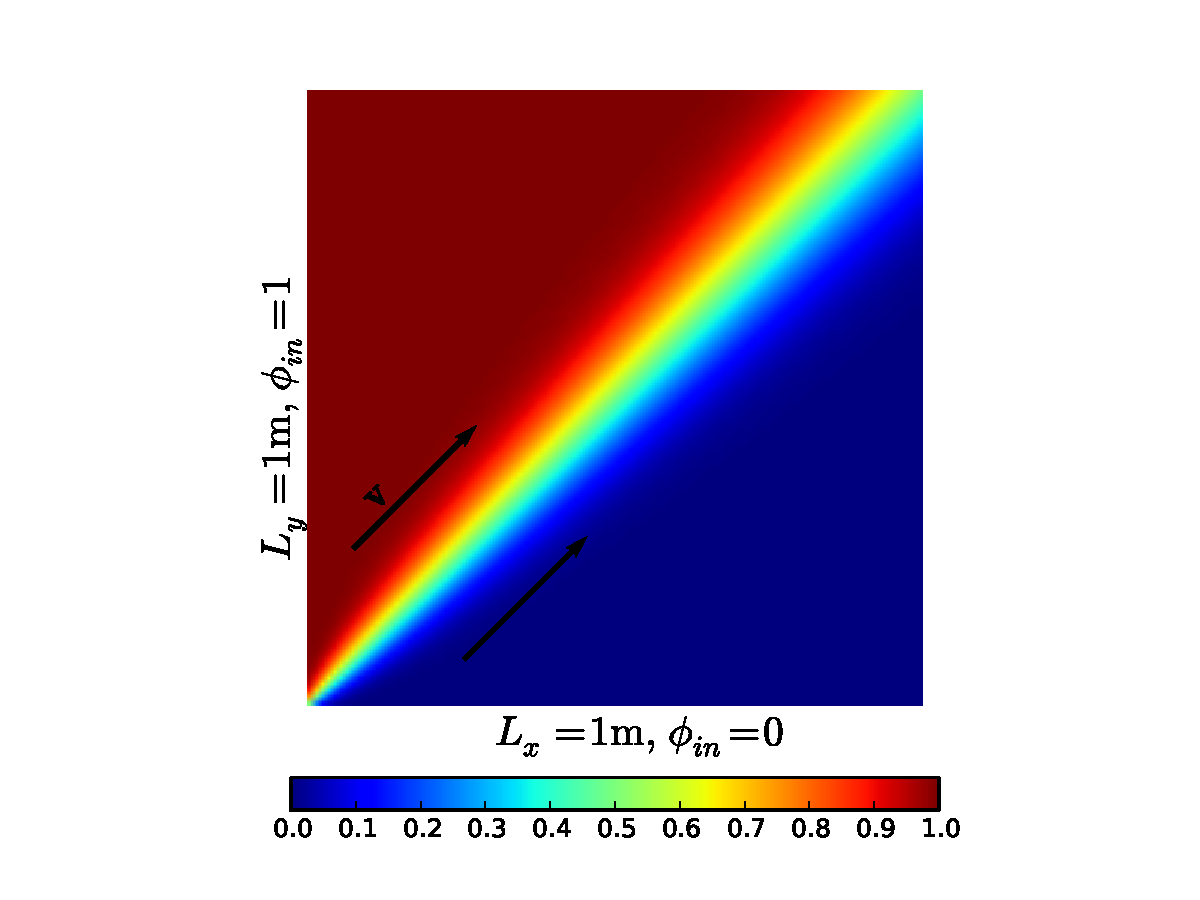
\includegraphics[width=1\linewidth]{up101.pdf}
  \caption{The upwind scheme.}
  \label{fig:sub11}
\end{subfigure}%
\begin{subfigure}{0.5\textwidth}
  \centering
  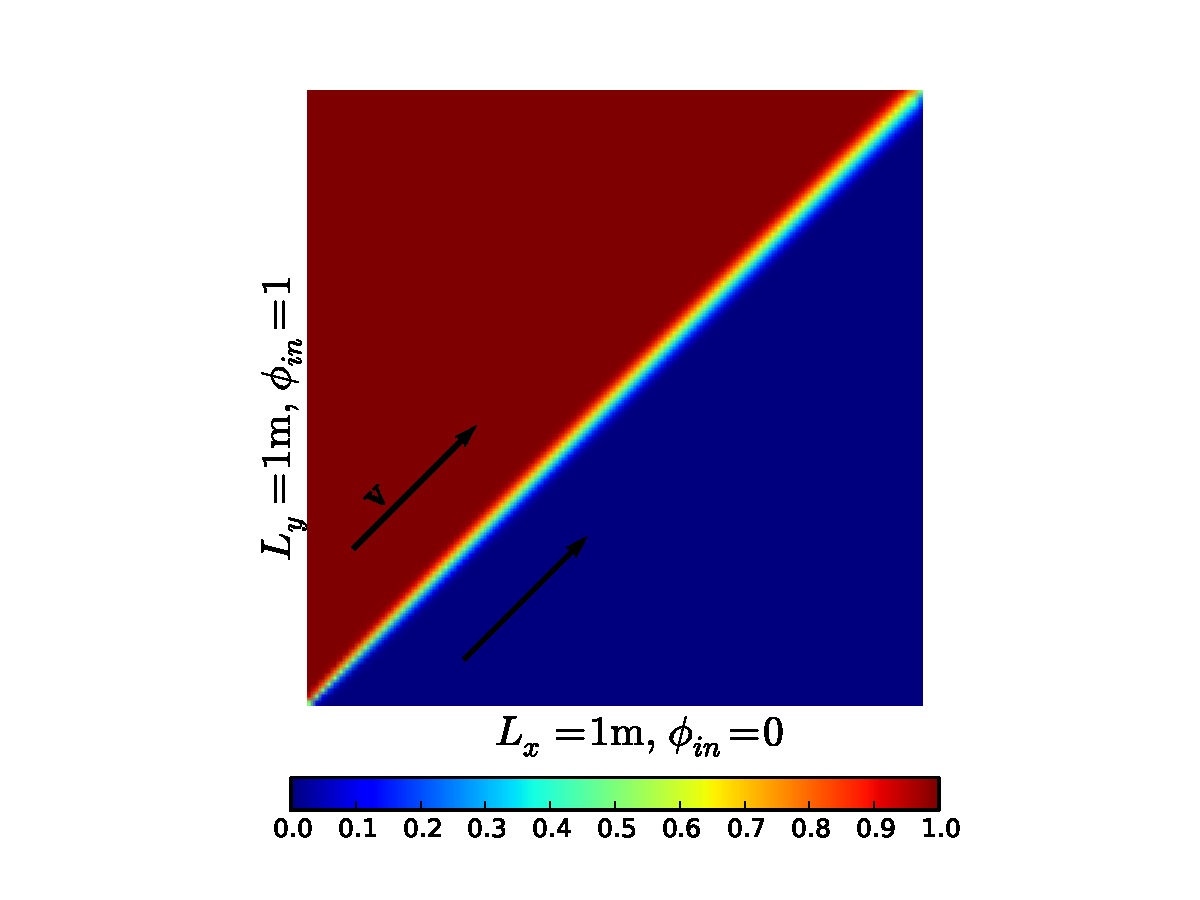
\includegraphics[width=1\linewidth]{smart101.pdf}
  \caption{The smart scheme.}
  \label{fig:sub2}
\end{subfigure}
\caption{The variable $\phi$ distribution over the computational domain using a grid size of 100x100 for the upwind and smart convection schemes and a velocity field $\textbf{v}=\cos\frac{\pi}{4}\textbf{i}+\sin\frac{\pi}{4}\textbf{j}$.}
\label{fig:sub22}
\end{figure}
We can observe that the results are smoother and more accurate in the case of a fine mesh of 100x100 grid size. Note that the smart scheme is more accurate because it takes into account the one dimensionality in the $i$ and $j$ directions used in the upwind scheme when choosing the upwind nodes.

\section*{Additional Case and Results}
In this section, and since the code developped is a general code, I will show 1 addition case where $\textbf{v}=\cos\frac{\pi}{4}\textbf{i}-\sin\frac{\pi}{4}\textbf{j}$. Now the north and west faces are inlets and the east and south are outlets.
\makeatletter
\setlength{\@fptop}{0pt}
\makeatother
\begin{figure}[ht!]
\centering
\begin{subfigure}{0.5\textwidth}
  \centering
  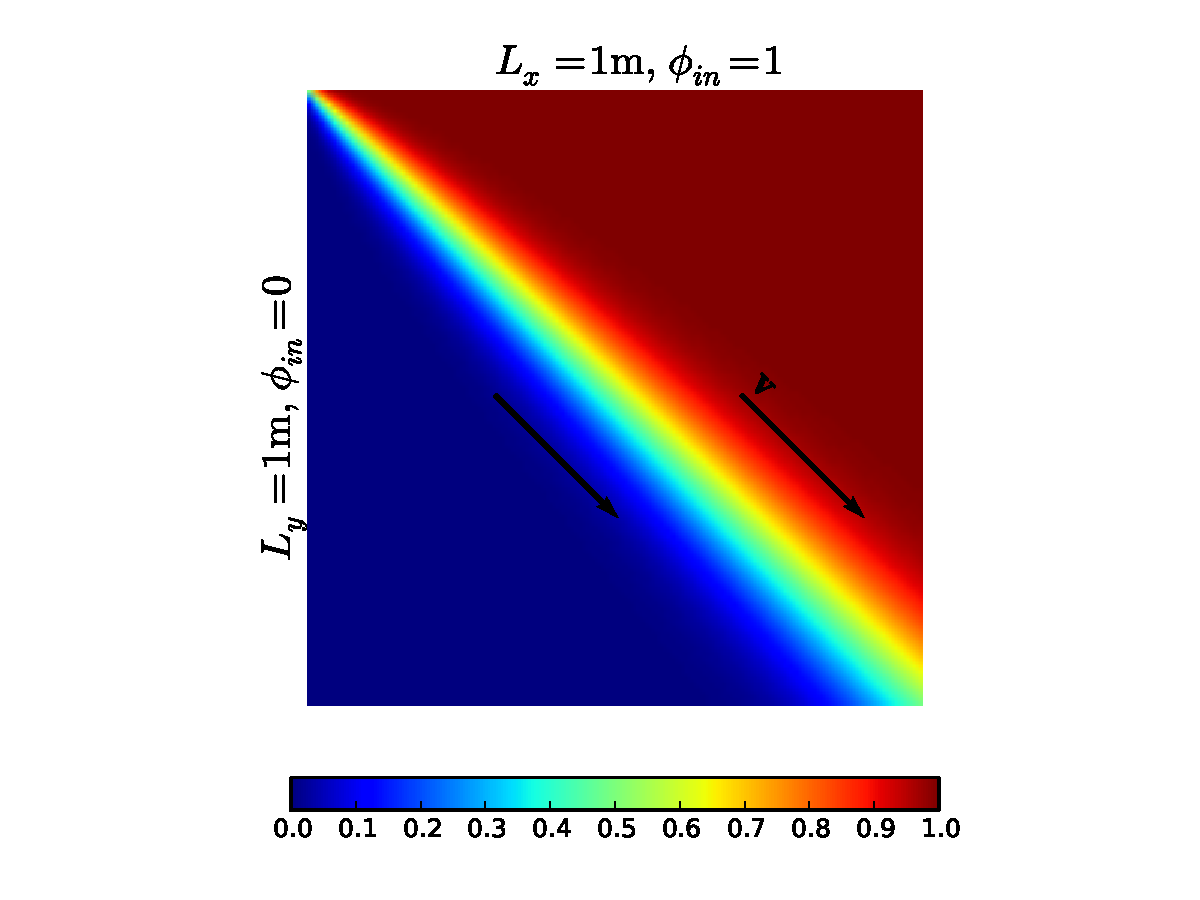
\includegraphics[width=1\linewidth]{addUp.pdf}
  \caption{The upwind scheme.}
  \label{fig:sub31}
\end{subfigure}%
\begin{subfigure}{0.5\textwidth}
  \centering
  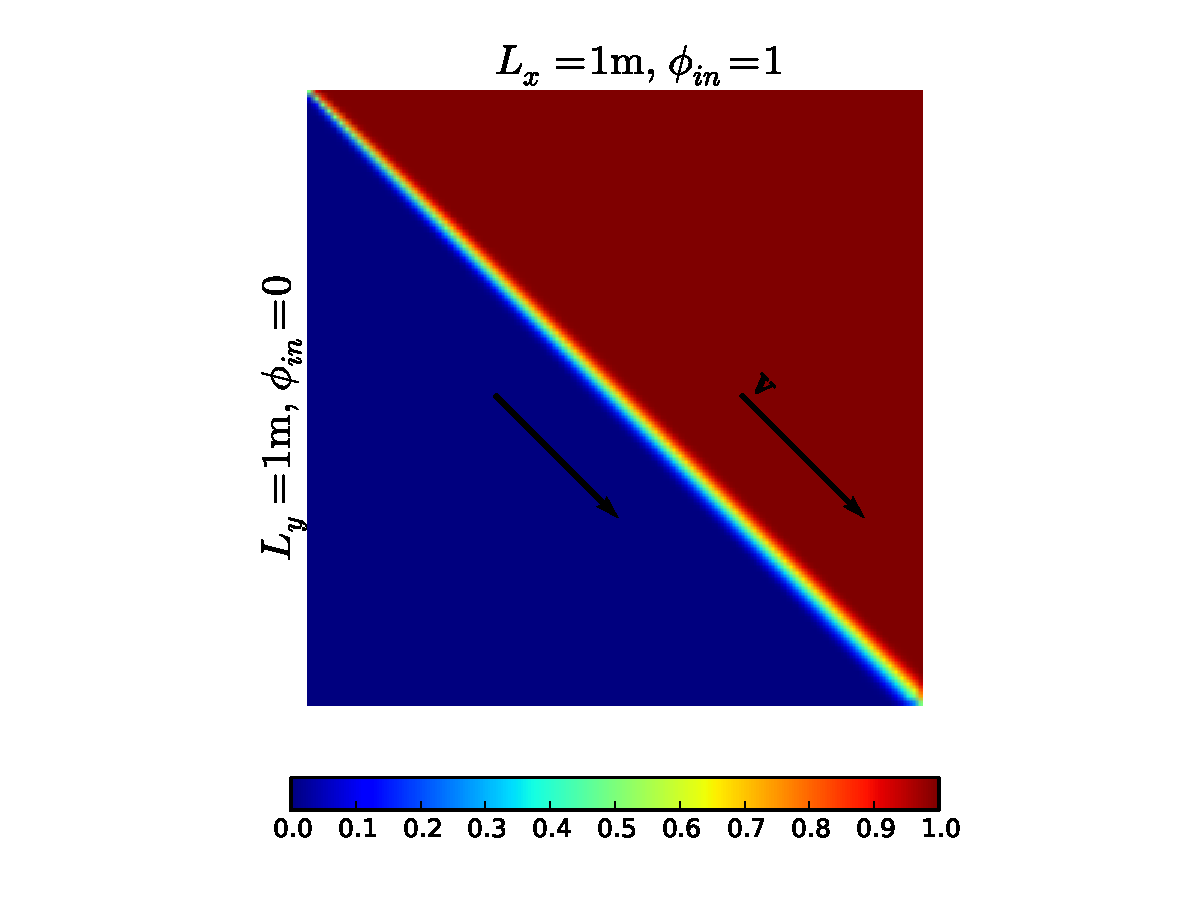
\includegraphics[width=1\linewidth]{addSmart.pdf}
  \caption{The smart scheme.}
  \label{fig:sub2}
\end{subfigure}
\caption{The variable $\phi$ distribution over the computational domain using a grid size of 100x100 for the upwind and smart convection schemes and a velocity field $\textbf{v}=\cos\frac{\pi}{4}\textbf{i}-\sin\frac{\pi}{4}\textbf{j}$.}
\label{fig:sub32}
\end{figure}
\end{document}

